
\iffalse
\begin{figure*}[ht]
    \centering
    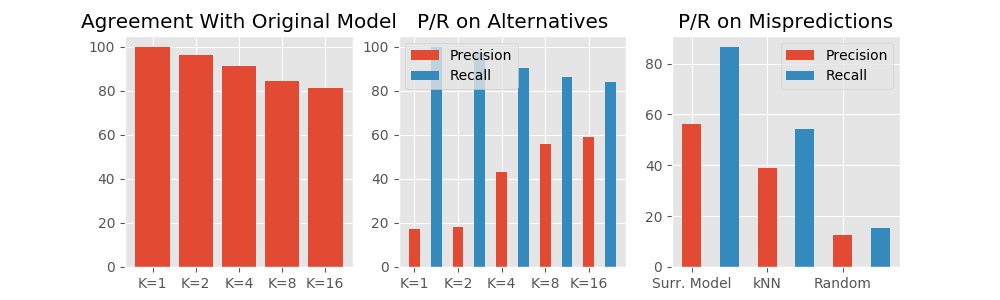
\includegraphics[width=\textwidth]{figures/result1.png}
    \caption{(A) Illustrates how a \sys  model can approximate a complex model, (B) illustrates how well this surrogate model can isolate mispredictions in terms of precision and recall, and (C) why alternative approaches do not work.}
    \label{fig:teaser}
\end{figure*}
\fi

\section{Experimental Results}
This section presents key experimental results  that highlight use cases where \sys models can help identify training data that causes mispredictions, 
when \sys diverges from the user's more complex model, and a comparison with alternative explanation approaches based on \ewu{nearest-neighbors or classification}.

\subsection{Datasets}
We split each dataset into a training dataset $80\%$ and test dataset $20\%$. 

\stitle{Movie: } We have a dataset of movie descriptions IMDB~\footnote{ \url{ftp://ftp.fu-berlin.de/pub/misc/movies/database/}} and Yahoo~\footnote{ \url{http://webscope.sandbox.yahoo.com/catalog.php?datatype=r}}.
Each movie has a title, a short 1-2 paragraph plot description, year, rating, language, and a list of categories, and the goal is to train a model to predict whether a movie is a ``Horror'' or ``Comedy'' from the description and title.  
The total dataset has 506,244 records.
First, using TensorFlow, we trained a LSTM-based model to predict these categories. The first layer of this model computes what is called a word-embedding, where the LSTM learns a feature-space in which similar words (co-occuring) are closer together. 
The next two layers consist of dense layers that map the words from the feature-space to classification outputs.
The result is a model that achieves 93\% accuracy, which is far more accurate than simpler alternatives on a Bag-of-Words featurization (random forests 90\%, Linear SVM 81\%, Kernel SVM 85\%).

\stitle{Fraud: } ProPublica collected a dataset of corporate donations to medical researchers to analyze conflicts of interest~\cite{dollarsfordocs}. 
Records contain the PI's medical specialty, the drug brand name (null if not drug), the device brand name (null if not a device), name of pharamceutical donor, the amount donated, and whether the research is disputed.
The dataset comes with a \texttt{status} field that describes whether or not the donation was allowed under the declared research protocol.
We used a Multi-Layer Perceptron to classify disallowed donations which achieved a 82\% accuracy (random forest 81\%, Linear SVM 80\%, Kernel SVM 80\%).

\subsection{Experiments}

\begin{figure}[ht]
    \centering
    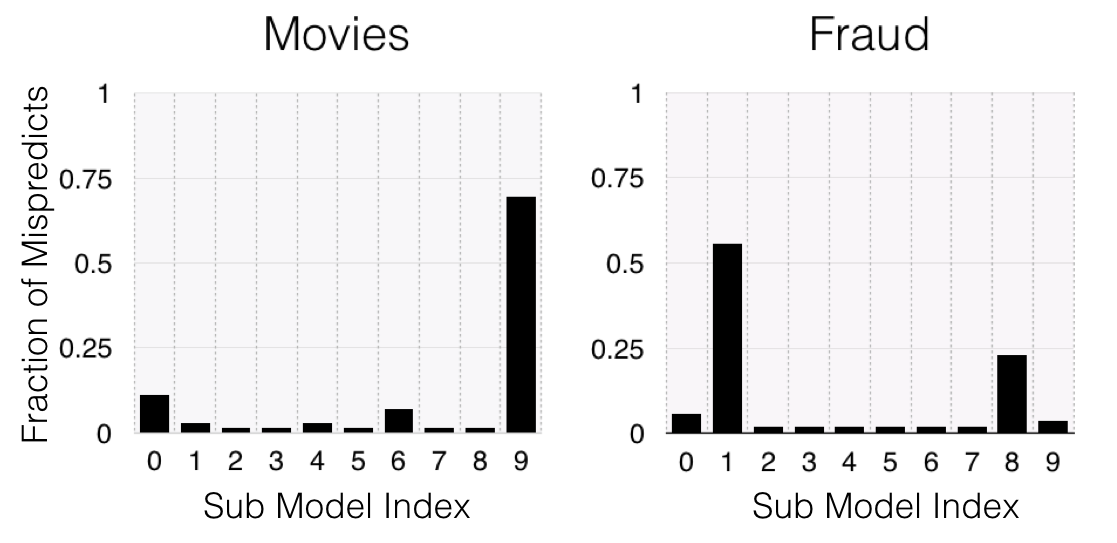
\includegraphics[width=\columnwidth]{figures/concentration.png}
    \caption{On two datasets, we show how mispredictions concentrate around specific submodels. This means there are specific regions of the feature-space most associated with mispredictions.}
    \label{fig:concentrate}
\end{figure}

\stitle{Exp 1. Isolating Mispredictions }  
In the first experiment, we explore whether mispredictions concentrate around particular submodels. We train the models on 80\% of the dataset, and test on the remaining 20\%. We measure the fraction of mispredictions attributed to each submodel. We want to show that mispredictions concentrate around specific submodels and are not evenly distributed throughout the feature-space. Figure \ref{fig:concentrate} shows this effect when we apply our algorithm to approximate the Movie and Fraud models with $k=10$ submodels. For the Movie dataset, 70\% of the mis-predictions are attributed to a single submodel.
For the Fraud dataset, 78\% of the errors are attributed to two of the submodels.

\begin{figure}[ht]
    \centering
    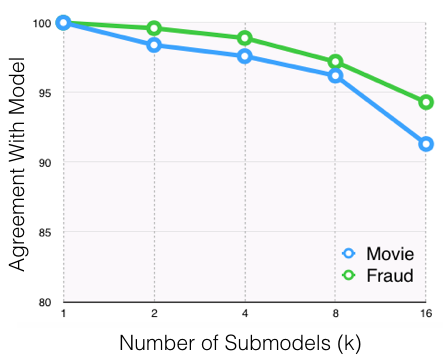
\includegraphics[width=0.6\columnwidth]{figures/agreement.png}
    \caption{On two datasets, we find that the discretized models agree with greater than 90\% accuracy with the original model. As the number of submodels increase the accuracy goes down.}
    \label{fig:agreement}
\end{figure}

\stitle{Exp 2. Agreement With the Original Model}
We now measure the agreement between the \sys model with the original model as we increasing the number of partitions $k$ (Figure~\ref{fig:agreement}, where agreement is the accuracy with respect to the original model.
We find that with $k=16$, both \sys models still retain $>90\%$ agreement with the original model.
\ewu{SANJAY CHECK:} This suggests that \sys can help developers identify more precise subsets of the training data while still trusting that the \sys models are reflective of the original model.


\stitle{Exp 3. Faster and More Accurate than Nearest Neighbors}  
An alternative approach is to find training data that are nearby neighbors of the mispredicted test point\ewu{, or to train a decision tree directly on the correctly and incorrectly classified test points}, however each approach has their drawbacks.
For the nearest neighbors approach, it is possible to quickly find the neighbors by using intelligent indexing structures such as KD-trees or Oct-trees.  However spatial indices are well known to have difficulty scaling to very high dimensional datasets.  \ewu{In addition, finding the neighbors in a high dimensional space may simply not identify relevant results.
The classification approach is fast, however it ignores the user's original model and may also identify spurious rules.}
On the other hand, \sys is explicitly designed to mimic the user's model, and the decision tree learned by the meta-modelcan easily be used to index or partition the training data can be indexed.
Our approach returns more than 20x faster than a nearest neighbor search even when coupled with dimensionality reduction and a KD-Tree \ewu{talk about quality of results and compare with classification.}

\begin{table}[ht!]
\centering
\caption{Runtimes of the different algorithms}
\label{my-label}
\begin{tabular}{lll}
Algorithm & Movie & Fraud \\ \hline
kNN & 35.61 & 22.11  \\
kNN+PCA & 12.34 & 8.97  \\
Ours & 0.534 & 0.31 
\end{tabular}
\end{table}

